\documentclass[tikz]{standalone}
\usepackage{pgfplots}
\begin{document}

% \begin{tikzpicture}
% \begin{axis}[
%     symbolic x coords={com.facebook.katana,com.android.vending,com.google.android.gms,com.google.android.backuptransport,com.google.android.gsf.login,com.google.android.gsf,com.google.android.youtube,com.facebook.orca,com.cleanmaster.mguard,com.instagram.android,com.estrongs.android.pop,com.enflick.android.TextNow,org.telegram.messenger,com.samsung.android.scloud,com.weather.Weather,com.whatsapp,com.google.android.googlequicksearchbox,com.google.android.syncadapters.contacts,com.tencent.mm,com.google.android.gm,com.samsung.android.email.provider,},
%     xtick=data,
%     width=10cm,
%     height=5cm,
%     x tick label style={rotate=90, anchor=east},
%     scaled y ticks=real:1,
%     ytick scale label code/.code={}
%     ]
%     \addplot[ybar,fill=blue] coordinates {
%         (com.facebook.katana,28515)
%         (com.enflick.android.TextNow,12076)
%         (com.google.android.youtube,11817)
%         (com.cleanmaster.mguard,10975)
%         (com.estrongs.android.pop,7783)
%         (com.google.android.gms,6708)
%         (com.google.android.backuptransport,6702)
%         (com.google.android.gsf,6655)
%         (com.google.android.googlequicksearchbox,6489)
%         (com.google.android.gsf.login,6463)
%         (com.google.android.syncadapters.contacts,3988)
%         (com.weather.Weather,3927)
%         (com.android.vending,3747)
%         (com.whatsapp,3601)
%         (com.google.android.gm,2769)
%         (com.samsung.android.email.provider,2296)
%         (com.instagram.android,2217)
%         (com.facebook.orca,1855)
%         (com.samsung.android.scloud,1562)
%         (com.tencent.mm,1539)
%         (org.telegram.messenger,633)
%     };
% \end{axis}
% \end{tikzpicture}

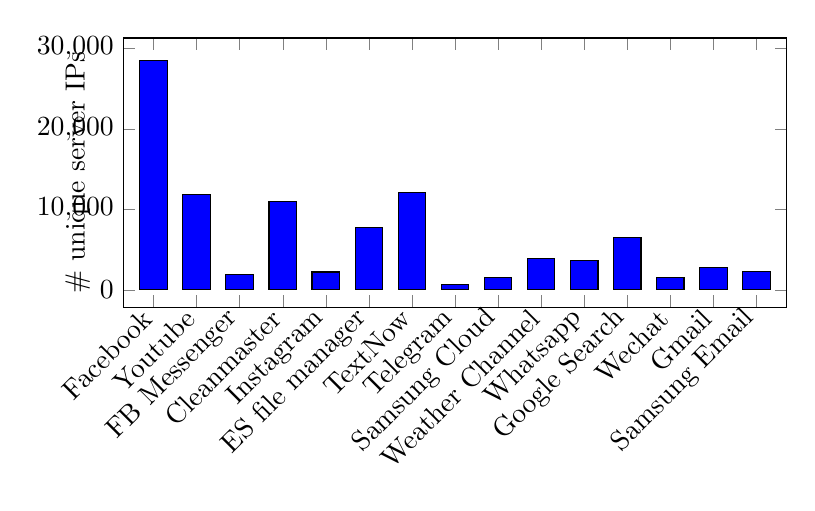
\begin{tikzpicture}
    \begin{axis}[
        symbolic x coords={Facebook,Youtube,FB Messenger,Cleanmaster,Instagram,ES file manager,TextNow,Telegram,Samsung Cloud,Weather Channel,Whatsapp,Google Search,Wechat,Gmail,Samsung Email},
        xtick=data,
        width=10cm,
        height=5cm,
        x tick label style={rotate=45, anchor=east},
        scaled y ticks=real:1,
        ytick scale label code/.code={},
        ylabel=\# unique server IPs,
        ylabel style={at={(-2ex, 0.5)}},
        enlarge x limits=0.05
        ]
        \addplot[ybar,fill=blue] coordinates {
            (Facebook,28515)
            (TextNow,12076)
            (Youtube,11817)
            (Cleanmaster,10975)
            (ES file manager,7783)
            (Google Search,6489)
            (Weather Channel,3927)
            (Whatsapp,3601)
            (Gmail,2769)
            (Samsung Email,2296)
            (Instagram,2217)
            (FB Messenger,1855)
            (Samsung Cloud,1562)
            (Wechat,1539)
            (Telegram,633)
        };
    \end{axis}
    \end{tikzpicture}

\end{document}
